\documentclass{article}%scrartd
\usepackage{graphicx}
\usepackage{amsmath}
\begin{document}
\section{Phasenangeschnittenen Strom messen}
Im Labor soll nun ein phasenangeschnittener Strom gemessen und mit der DFT untersucht werden.
Dazu wird der Dimmer auf dem "Lampenbrett" verwendet.
\subsection{Versuchsaufbau}
Allgemein gilt: Um Strom zu messen muss man ein Amperemeter in Reihe mit der Last schalten. Daher muss auch hier der Stromwandler aus der "blauen Box" in Reihe zur Last geschaltet werden. Das in eine Spannung gewandelte und gefilterte Signal wird mit dem Sensorknoten gemessen. Das Messsignal wird anschließend mit Matlab weiterverarbeitet.
\begin{figure}[htb]
\centering
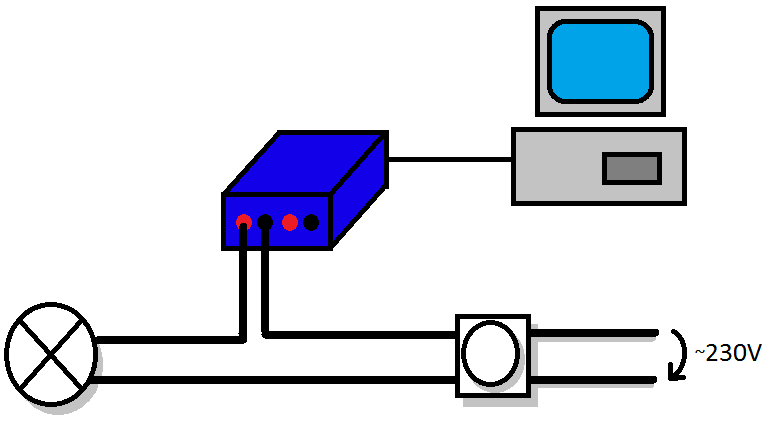
\includegraphics[width=1\textwidth]{Versuchsaufbau1.png}
\caption{Versuchsaubau um angeschnittenen Strom zu messen}
\end{figure}
\subsection{Versuchsdurchführung}
\subsubsection{Phasenanschnitt messen}
An dem Phasenanschnittdimmer wird ein Zündwinkel eingestellt. Dieser kann aber nicht am Dimmer bestimmt werden, da eine Skala fehlt. Statt dessen wird das Phasenangeschnittene Signal zunächst mit dem Ossziloskop gemessen. Dabei wird die Zeitdifferenz zwischen dem Nulldurchgang und Zündmoment gemessen. Anschließend wird das Signal auch mit dem Sensorknoten abgetastet.
Es werden Messpunkte bei vielfachen von ca. 2,5ms Phasenverschub aufgenommen. Anschließend wird ein Matlabskript geschrieben, dass den Zündwinkel aus den Messwerten bestimmt.\\ Um den Leckeffekt von vornerein zu umgehen, wird als Messdauer ein ganzzahliges vielfaches der Signalperiode (20ms) gewählt.\\ Die Abtastfrequenz muss wie folgt gewählt werden. Die 3dB-Grenzfrequenz des Allaisingfilters liegt bei 3,1kHz, die Auflösung des ADUs beträgt 10Bit und der Eingangsspannungsbereich beträgt 14V.\\
\begin{align}
U_{LSB} = \frac{14V}{2^{10}-1} = 0,01368V 
\end{align} 
Nun kann die benötigte Dämpfung, um Allaising zu verhindern, berechnet werden.\\
\begin{align}
D = 20 \cdot log_{10}(\frac{14V}{U_{LSB}}) = 60dB
\end{align} 
Der Filter ist ein Filter 8.Ordnung und besitzt eine Steilheit von 160dB/Dekade. Es wird abgeschätzt, dass der Filter ab ca.3,5kHz um über 60dB dämpft. Daher muss die Abtastfrequenz mindestens 7kHz betragen.
\subsubsection{Auswirkungen des Fensters}
Es werden nun nacheinander Rechteck-, Hanning- und Blackmanfenster über das Signal gelegt. Die Längen der Fenster sind absichtlich so gewählt, dass es zum leckeffekt kommt. Es wird nun untersucht, wie sich die unterschiedlichen Fenster auf den Leckeffekt auswirken. 
\subsubsection{Qualität der Netzspannung}
Nun soll die Qualität der Netzspannung überprüft werden. Theoretisch beträgt die Netzspannung 230V bei 50Hz. Allerdings können auf der Grundwelle zusätzlich zu den 50Hz weitere Oberwellen vorhanden sein. Der Anteil dieser Oberwellen an der Versorgungsspannung darf nicht über $8\%$ liegen.\\Für diesen Versuch wird die Netzspannung an den Spannungswandler der Blauenbox angelegt. Nun kann mit dem Sensorknoten die Netzspannung gemessen werden. Der Spannungswandler setzt die Eingangsspannung um den Faktor 56,6 herrab. Um die Netzspannung zu bestimmen, muss der Messwert mit 56,6 multipliziert werden.
\begin{figure}[htb]
\centering
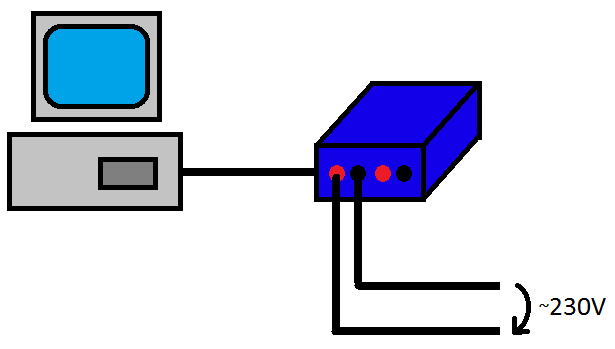
\includegraphics[width=1\textwidth]{Versuchsaufbau2.png}
\caption{Versuchsaubau um Netzqualität zu messen}
\end{figure}
\end{document}